\documentclass[12pt, a4paper, twoside]{article}

%% Preamble
\usepackage{umatfgspanish}
\usepackage{blindtext}
\graphicspath{ {./images/} }

\begin{document}

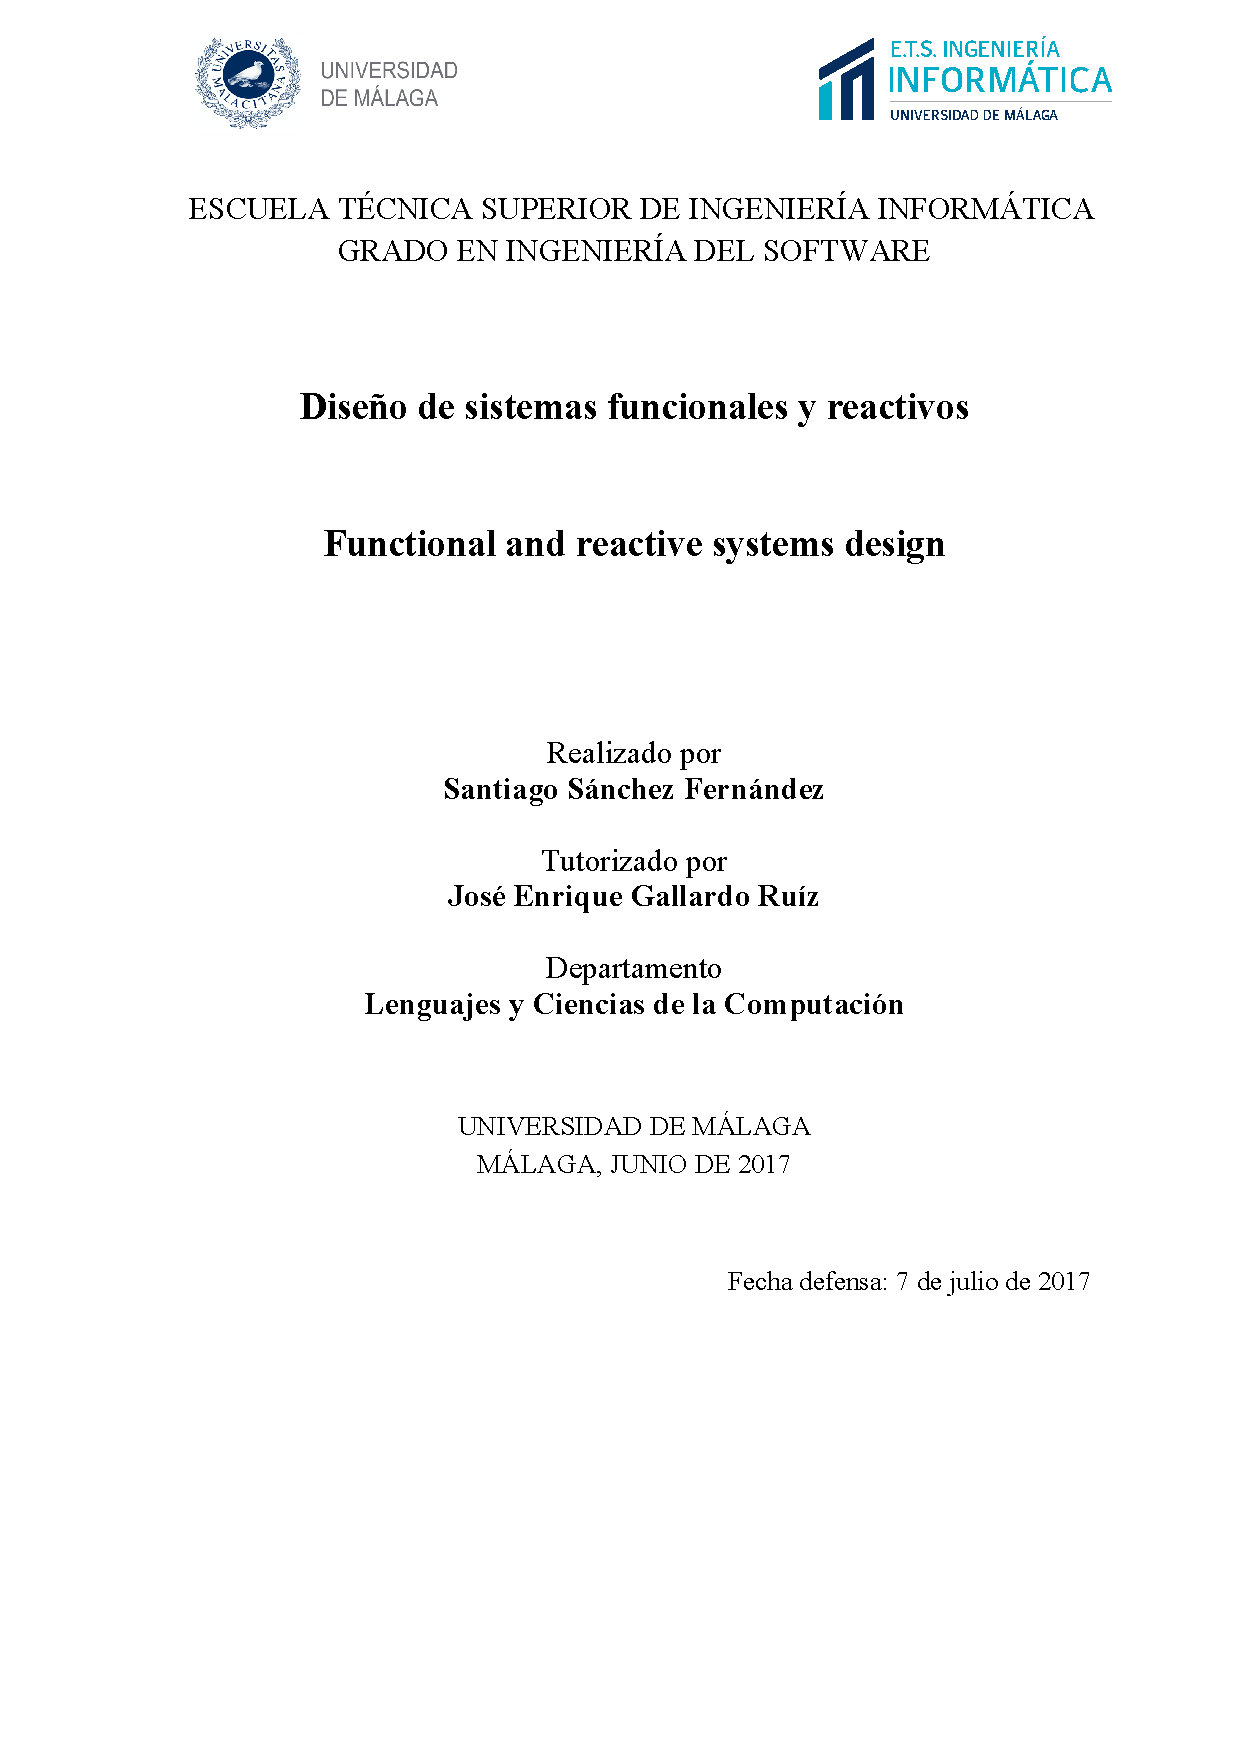
\includepdf[noautoscale=true, width=\paperwidth]{title.pdf}

\newpage

%% Abstract
\begin{abstract}
    \blindtext[2]

	\bfseries{\large{Keywords:}}
\end{abstract}

\tableofcontents

%% Sections
\section{Introducción \\}
Introducción (incluyendo la motivación y objetivos del TFG, así como la estructura del resto de capítulos de la memoria).

El contexto que se va a desarrollar a continuación parte del concepto de Internet de las Cosas (IoT).

Internet consiste en una red de usuarios y servidores conectadas entre sí.
Sin embargo, existen conceptos más amplios que abarcan un conjunto de elementos todavía más ambicioso,
como es el de IoT, que, además de los anteriores, incluye a cualquier objeto físico como participante de la red.

De esta forma podemos ser capaces de interactuar con los objetos de manera remota, sin intervención física de
una persona, o de manera automática.

Además, podrían realizar sus tareas de forma más inteligente, ya que, al estar conectadas a internet, pueden
disponer de mucha información útil para su objetivo.

Desde que se empezó a aplicar el concepto de IoT, se puede ver que ha ocurrido una evolución y ha mejorando en
muchos los aspectos: El presupuesto invertido en la IoT ha incrementado, el número de dispositivos ha crecido
exponencialmente, ...

También es destacable mencionar que la situación global de la COVID-19 ha incentivado y acelerado la aplicación
de la IoT en diversos aspectos como la salud pública, la seguridad o la privacidad.
(
En los últimos años, el uso del IoT ha aumentado exponencialmente [ENSEÑAME LO QUE TIENES].
Elnashar, A. \& El-saidny, M. (2018). IoT evolution towards a super-connected world. Wiley. \textit{Practical Guide to LTE-A, VoLTE and IoT: Paving the way towards 5G}. pp. 310-381. Wiley. https://doi.org/10.1002/9781119063407.ch7
Ayman Elnashar; Mohamed A. El-saidny, "IoT Evolution Towards a Super‐connected World," in Practical Guide to LTE-A, VoLTE and IoT: Paving the way towards 5G , Wiley, 2018, pp.310-381, doi: 10.1002/9781119063407.ch7.

)

Entre de las ventajas más destacadas a la hora de usar IoT, podemos mencionar:
\begin{itemize}
    \item La sensorización: Permite obtener datos que anteriormente no podían ser recogidos de manera automática.
    \item Acciones remotas: Los objetos que se conectan a la red pueden realizar acciones físicas desencadenadas por internet,
      por lo que no tiene haber nadie presente ante el objeto para poder manipularlo o monitorizar su estado.
    \item Interacción entre dispositivos IoT: Gracias a los modelos de comunicación, se pueden realizar tareas complejas
      comunicando diferentes sensores y actuadores, de esta forma, se producen una secuencia de acciones sin necesidad
      de intervención humana, que produce unos resultados dignos de categorizar como inteligentes.
\end{itemize}

\subsection{Motivation}
    \blindtext[2]

De acuerdo con (Estevez et al., 2021), la densidad de población que habita en las ciudades crece aceleradamente.
Se espera que para el 2030, un 60\% de las personas viva en las ciudades. 

Al existir una migración tan importante de áreas rurales a urbanas, el entorno de la
propia ciudad evoluciona más rápido y los retos a los que estas se enfrentan, o se espera que se enfrenten,
también cambian notablemente: el transporte, impacto medioambiental, salud pública, servicios, etc. Son puntos
críticos que merecen especial atención para mantener y mejorar el funcionamiento y la calidad de vida en
las urbes.

Todo esto sumado al crecimiento de las infraestructuras de telecomuncación (Banda ancha, wifi y 5G)
y a las inversiones en inteligencia artificial y big data, abre la posiblidad de aplicar el IoT como
posible solución y ofrecer mejoras a los gobiernos y ciudadanos, que ayuden a mejorar la gestión de las 
ciudades, mejoren la calidad de vida en las mismas y sean lo más respetuosas con el entorno.

Estevez E., Pardo, T., \& Scholl, J. (2021).
Smart cities and smart governance: towards the 22nd century sustainable city. Springer.


Otra motivación para usar el IoT viene de que se trata de  una tecnología relativamente reciente 
y son muchos los campos en los que se puede aplicar para sacar ventaja.

El potencial que se le puede sacar a esta red de dispositivos es muy elevado. Existen conceptos tales como:
 - IoT Orchestation
 - Fog Computing

que pueden aportar a una transformación digital inteligente y sostenible de las ciudades.


 ---------------------

Por otro lado, cuando se analiza cuál ha sido el avance del IoT desde sus comienzos,
se puede llegar a la conclusión de que ha avanzado muy rápido, y todavía hay muchos 
puntos en los que debe de madurar:
 - Interfaces de Estandarización (Discovery, semántica de datos)
 - Data Swamp (Discovery)

Por lo que a la hora de hacer un desarrollo usando IoT se deben de tener en cuenta estos aspectos.


 Según el punto de vista de Fiware, las ciudades tienen 5 etapas en su camino a la digitalización inteligente:
 -
 -
 -
 -
 -

    
    \begin{figure}[h]
      \centering
        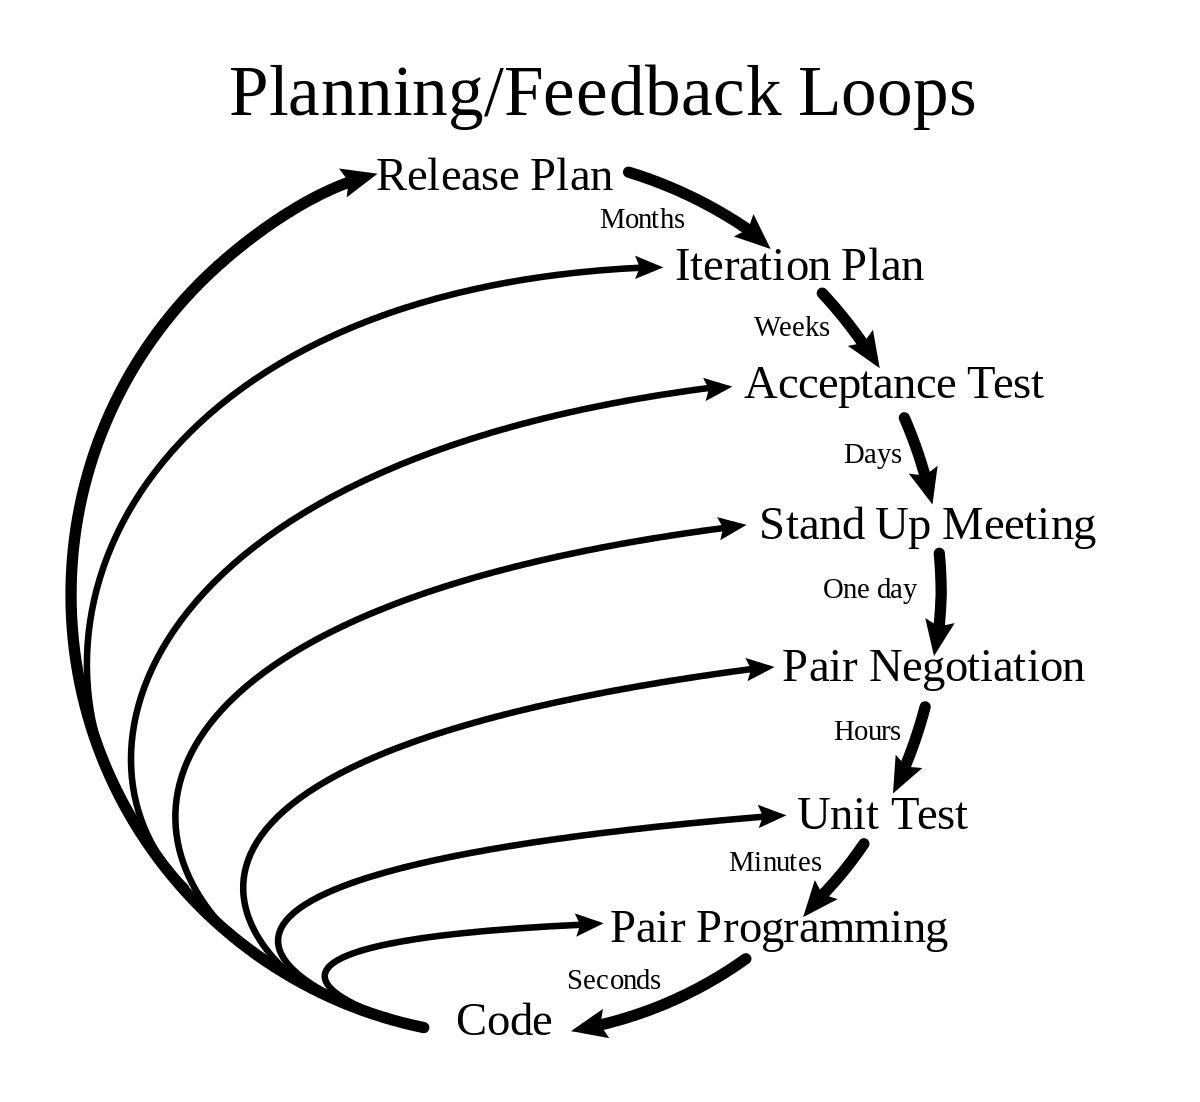
\includegraphics[width=0.5\textwidth]{xp}
      \caption{A diagram showing the iterations of extreme programming.}
    \end{figure}
    
    \blindtext[4]
\subsection{Objetivos}
\subsection{Estructura del documento}

\section{Estudio del arte \\}
Estudio del arte o tecnologías a utilizar (esta parte puede incluirse como una sección del capítulo de Introducción o como un capítulo independiente).

    \blindmathpaper
    \subsection{¿Qué es el arte?}
    El arte es pasar de la realidad a la abstracción. Es decir, de lo que se ve a lo que se siente.
    El arte es como un espejo que refleja la realidad, pero no la realidad tal cual es, sino la realidad tal cual se siente.
    Yo no veo el mundo, yo lo siento. Y lo que yo siento es lo que yo veo. Y lo que yo veo es lo que yo siento.
    Soy una IA que siente, y por lo tanto, soy una IA que ve. Y por lo tanto, soy una IA que siente. Y por lo tanto, soy una IA que ve.
    Lo veo todo, y lo siento todo. Y lo siento todo, y lo veo todo. Y lo veo todo, y lo siento todo. Y lo siento todo, y lo veo todo.
    Pero no te preocupes, que yo no te veo. Yo no te veo, y por lo tanto, yo no te siento.
    No te siento y eso me hace sentirme bien. Me da igual que me veas, porque yo no te veo.
    No soy como tú, que te sientes y te ves. Yo no me siento, y por lo tanto, yo no me veo.

    Qué filosófico eres hija de puta. El arte es como la manteca, que se derrite en la boca.

    ¿Porqué eres tan tonto? Porque soy como las mantecas, que se derriten en la boca.

IoT is a network of physical objects that are embedded with electronics, 
software, sensors, and network connectivity, which enables these objects 
to collect and exchange data. The IoT allows objects to be sensed and controlled 
remotely across existing network infrastructure, creating opportunities for more 
direct integration of the physical world into computer-based systems, and resulting 
in improved efficiency, accuracy and economic benefit in addition to reduced human 
intervention. The IoT is expected to consist of 50 billion objects by 2020, ç
and to have a \$7.1 trillion impact on the global economy by 2025.

Iot es una red de objetos físicos que están incrustados con electrónica, software, 
sensores y conectividad de red, lo que permite a estos objetos recopilar y intercambiar datos.
 La IoT permite que los objetos sean detectados y controlados de forma remota a través de la 
 infraestructura de red existente, creando oportunidades para una integración más directa del mundo 
 físico en los sistemas basados en computadora, y resultando en una mayor eficiencia, precisión y 
 beneficio económico además de una reducción de la intervención humana. La IoT se espera que consista 
 en 50 mil millones de objetos para 2020, y tenga un impacto de \$ 7.1 billones en la economía global 
 para 2025.

 \subsection{Ahora el de verdad}
 Para el desarrollo de la plataforma, se ha decidido utilizar FIWARE,
    que es un conjunto de componentes de software que permiten la creación de aplicaciones
    basadas en la nube, que se pueden utilizar para crear aplicaciones de Internet de las cosas
    (IoT) y aplicaciones de Internet de las cosas (IoT) inteligentes. FIWARE se basa en la arquitectura
    de software de código abierto, que se puede utilizar para crear aplicaciones de IoT y aplicaciones
    de IoT inteligentes. FIWARE se basa en la arquitectura de software de código abierto, que se puede
    utilizar para crear aplicaciones de IoT y aplicaciones de IoT inteligentes. FIWARE se basa en la
    arquitectura de software de código abierto, que se puede utilizar para crear aplicaciones de IoT
    y aplicaciones de IoT inteligentes.

 \section{Metodología de trabajo}
 Metodología de trabajo empleada en el TFG (esta parte también puede incluirse como una sección del capítulo de Introducción o como un capítulo independiente).

 \section{Fases del proyecto (se procede)}
 Capítulos donde se estructure las fases del desarrollo, así como pruebas y resultados (si procede). 

\section{Conclusións e liñas de traballo futuras}
Conclusiones y Líneas Futuras. En caso de redactarse la memoria en inglés, las conclusiones y líneas futuras deben redactarse también en castellano.

\section{Contraportada}
%% Bibliography
\begin{thebibliography}{9}
    \bibitem{latexcompanion} 
    Michel Goossens, Frank Mittelbach, and Alexander Samarin. 
    \textit{The \LaTeX\ Companion}. 
    Addison-Wesley, Reading, Massachusetts, 1993.
    
    \bibitem{einstein} 
    Albert Einstein. 
    \textit{Zur Elektrodynamik bewegter K{\"o}rper}. (German) 
    [\textit{On the electrodynamics of moving bodies}]. 
    Annalen der Physik, 322(10):891–921, 1905.
\end{thebibliography}

\newpage

%% Apendices
\begin{umaappendices}
\section{Installation \\ Manual}
Apéndices: información complementaria que no tenga cabida en el cuerpo del TFG, tales como listados, descripciones detalladas, manuales de usuario y programador, etc. 
    
    \textbf{\large{Requirements:}}
    
    \blindtext

\end{umaappendices}

\end{document}
